\documentclass[a4paper]{scrartcl}

\usepackage[english]{babel}
\usepackage[utf8]{inputenc}
\usepackage{times}
\usepackage{graphicx}
\usepackage{url}
\usepackage[colorinlistoftodos]{todonotes}
\usepackage{multicol}
\usepackage{wrapfig}

% Look for images in ./images folder.
\graphicspath{{./images/}}

% Front page main information.
\title{\gamename}
\subtitle{Game Design Document}
\author{}
\date{\today}

\begin{document}

% Define the name of the game.
\newcommand{\gamename}{\emph{Ice Cream Factory}}

\maketitle

\section{About the game}
    In \gamename, you are responsible for assembling an ice cream production
    line. You must place the right machines along the conveyor belt and fill the
    orders correctly. But don't think this is going to be an easy task. You must
    find out clever solutions in order to produce the right types of ice cream
    with only a few devices path changers. Prepare yourself to face a delicious
    series of mind blowing puzzles.

\section{Description}
    Produce ice cream is a sweet business. So many flavors, so many toppings, so
    many combinations! Your job in \gamename is to plan the factory production
    line in such a way that only the right combinations are made.

    In each stage you will have a limited number of devices and a list ice cream
    types that your factory needs to produce. You must find a way of fulfill the
    stage requirements by placing path-changing devices, ice cream dosers and
    other machines along the conveyor belt.

    The belt fed with vessels which will travel all the way to the freezer. When
    a vessel reach a device, the machine will perform an action according to its
    type.

    \subsection{Input machines}
        \subsubsection{Ice cream pint}
            \begin{wrapfigure}{l}{0.1\textwidth}
                \vspace{-15pt}
                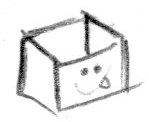
\includegraphics[scale=1]{devices/pint}
                \vspace{-20pt}
            \end{wrapfigure}

            Vessel for the regular ice cream. In some stages, the pint may have
            a bigger volume in order to be compatible with multiple runs through
            dosers.

        \subsubsection{Popsicle molds}
            \begin{wrapfigure}{l}{0.1\textwidth}
                \vspace{-15pt}
                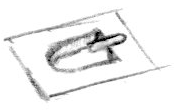
\includegraphics[scale=1]{devices/popsicle_molds}
                \vspace{-25pt}
            \end{wrapfigure}

            Vessel for the regular ice cream. In some stages, the pint may have
            a bigger volume in order to be compatible with multiple runs through
            dosers.

        \subsubsection{Banana plate}
            \begin{wrapfigure}{l}{0.1\textwidth}
                \vspace{-15pt}
                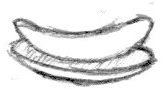
\includegraphics[scale=1]{devices/banana_plate}
                \vspace{-25pt}
            \end{wrapfigure}

            Vessel for the regular ice cream. In some stages, the pint may have
            a bigger volume in order to be compatible with multiple runs through
            dosers.

    \subsubsection{Action machines}
        \subsubsection{Ice cream doser}
            \begin{minipage}[t][6em][t]{\textwidth}
                \begin{wrapfigure}[5]{l}{0.16\textwidth}
                    \vspace{-20pt}
                    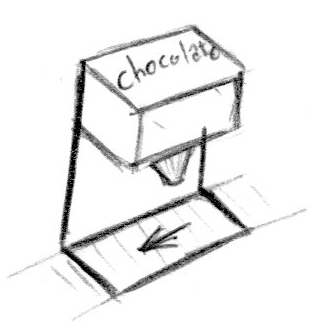
\includegraphics[scale=1]{devices/ice_cream_doser}
                    \vspace{-20pt}
                \end{wrapfigure}

                Vessel for the regular ice cream. In some stages, the pint may have
                a bigger volume in order to be compatible with multiple runs through
                dosers.
            \end{minipage}

        \subsubsection{Topping doser}
            \begin{minipage}[t][6em][t]{\textwidth}
                \begin{wrapfigure}[5]{l}{0.16\textwidth}
                    \vspace{-20pt}
                    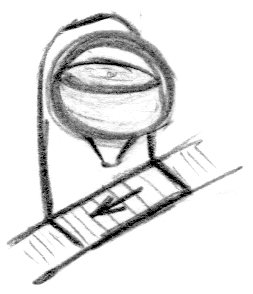
\includegraphics[scale=1]{devices/topping_doser}
                    \vspace{-10pt}
                \end{wrapfigure}

                Vessel for the regular ice cream. In some stages, the pint may have
                a bigger volume in order to be compatible with multiple runs through
                dosers.
            \end{minipage}

        \subsubsection{Special topping doser}
            \begin{minipage}[t][6em][t]{\textwidth}
                \begin{wrapfigure}{l}{0.2\textwidth}
                    \vspace{-20pt}
                    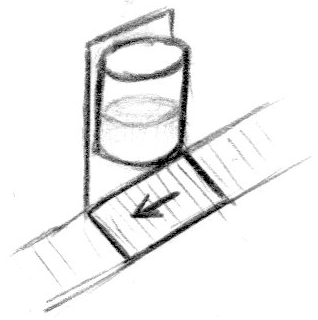
\includegraphics[scale=1]{devices/special_topping_doser}
                    \vspace{-20pt}
                \end{wrapfigure}

                Vessel for the regular ice cream. In some stages, the pint may have
                a bigger volume in order to be compatible with multiple runs through
                dosers.
            \end{minipage}

    \subsection{Control machines}
        \subsubsection{Switcher}
            \begin{minipage}[t][2em][t]{\textwidth}
                \begin{wrapfigure}{l}{0.2\textwidth}
                    \vspace{-20pt}
                    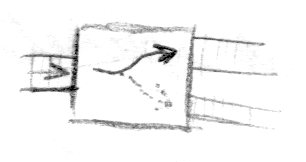
\includegraphics[scale=1]{devices/switcher}
                    \vspace{-20pt}
                \end{wrapfigure}

                Vessel for the regular ice cream. In some stages, the pint may have
                a bigger volume in order to be compatible with multiple runs through
                dosers.
            \end{minipage}

        \subsubsection{Weighing scale}
            \begin{minipage}[t][3em][t]{\textwidth}
                \begin{wrapfigure}{l}{0.2\textwidth}
                    \vspace{-20pt}
                    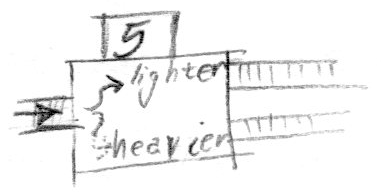
\includegraphics[scale=1]{devices/scale}
                    \vspace{-20pt}
                \end{wrapfigure}

                Vessel for the regular ice cream. In some stages, the pint may have
                a bigger volume in order to be compatible with multiple runs through
                dosers.
            \end{minipage}

        \subsubsection{Taster}
            \begin{minipage}[t][3em][t]{\textwidth}
                \begin{wrapfigure}{l}{0.24\textwidth}
                    \vspace{-20pt}
                    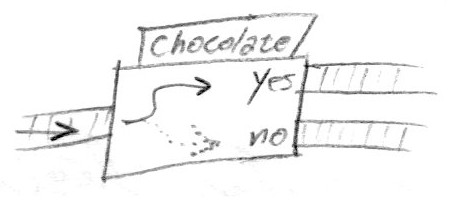
\includegraphics[scale=1]{devices/taster}
                    \vspace{-20pt}
                \end{wrapfigure}

                Vessel for the regular ice cream. In some stages, the pint may have
                a bigger volume in order to be compatible with multiple runs through
                dosers.
            \end{minipage}

        \subsubsection{Generic tester}
            \begin{minipage}[t][4em][t]{\textwidth}
                \begin{wrapfigure}{l}{0.45\textwidth}
                    \vspace{-20pt}
                    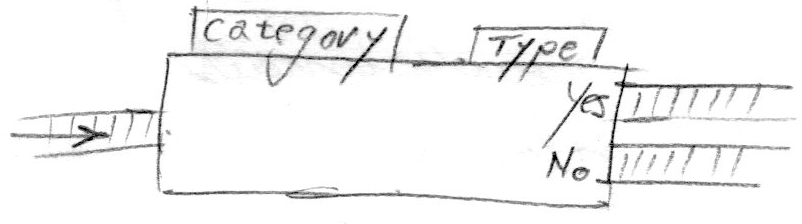
\includegraphics[scale=1]{devices/generic_conditional}
                    \vspace{-20pt}
                \end{wrapfigure}

                Vessel for the regular ice cream. In some stages, the pint may have
                a bigger volume in order to be compatible with multiple runs through
                dosers.
            \end{minipage}

        \subsubsection{Joint}
            \begin{minipage}[t][3em][t]{\textwidth}
                \begin{wrapfigure}{l}{0.2\textwidth}
                    \vspace{-20pt}
                    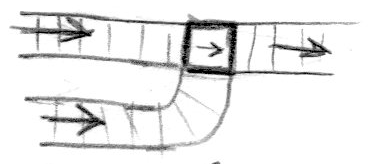
\includegraphics[scale=1]{devices/joint}
                    \vspace{-20pt}
                \end{wrapfigure}

                Vessel for the regular ice cream. In some stages, the pint may have
                a bigger volume in order to be compatible with multiple runs through
                dosers.
            \end{minipage}

    \subsection{Other}
        \subsubsection{Freezer}
            This is the end of line. All tracks must lead to the freezer so the
            ice cream can get ready to the costumers.

        \subsubsection{Synchronizer}

        \subsubsection{Logic gates}

\section{Features}
    \begin{itemize}
        \item Over XXX levels;
        \item 3 base ice creams, 4 flavors, 5 toppings, 4 special toppings;
        \item 13 different factory machines;
        \item Mind blowing puzzles;
    \end{itemize}

\section{Target platforms}
    \gamename is a simple and casual game, making it ideal for browser, tablets
    and PC. Player will perform actions through mouse clicking or by touch.

\section{Concept art}
    Here there are a few images to show the visual identity of \gamename.

    \centering
    $[$ TO BE FILLED $]$

\section{Similar games}
    In this section we can see some factory games which have the same conveyor
    concept present in \gamename.

    \begin{multicols}{2}
        \subsection{Cake Factory - Barbie Games}
            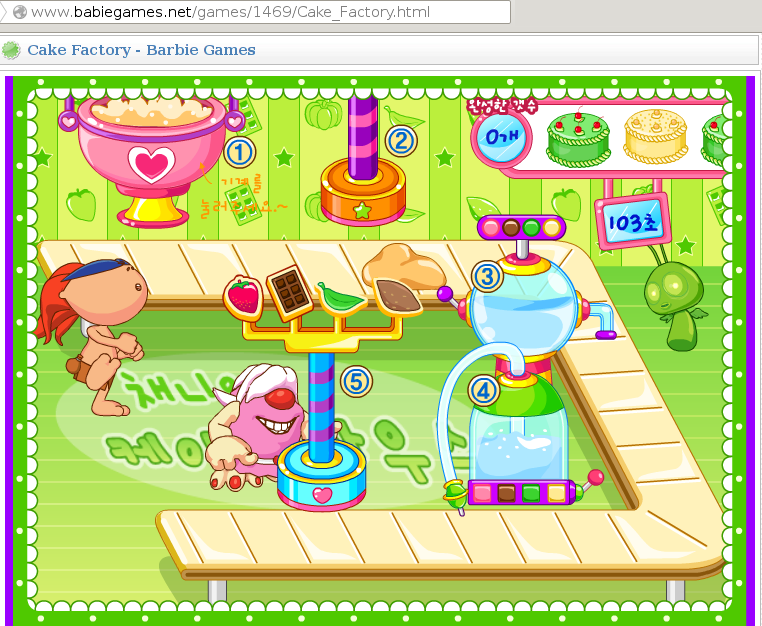
\includegraphics[width=0.49\textwidth]{similar_games/CakeFactory}

        \subsection{Toy Factory Fun}
            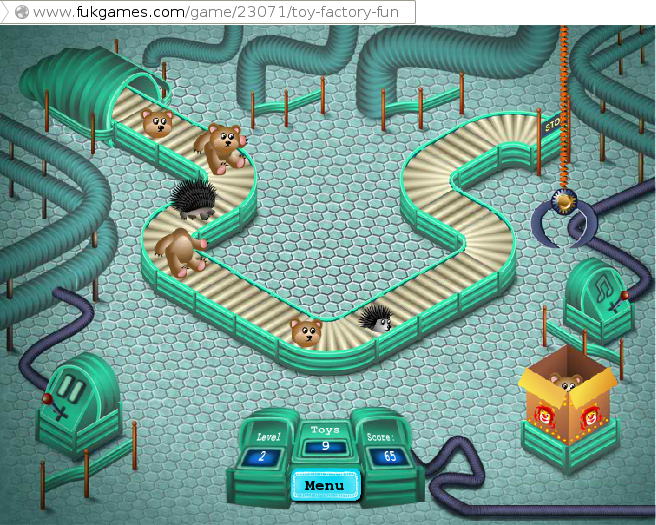
\includegraphics[width=0.49\textwidth]{similar_games/ToyFactoryFun}
    \end{multicols}

    \begin{multicols}{2}
        \subsection{Jewel Factory}
            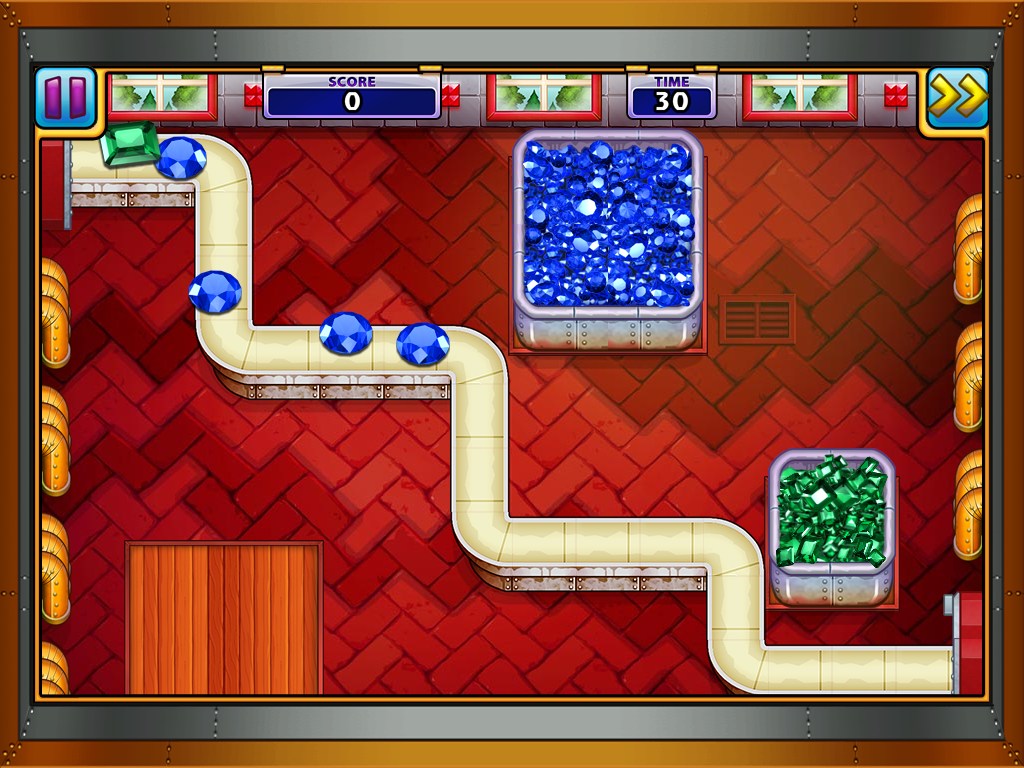
\includegraphics[width=0.49\textwidth]{similar_games/JewelFactory}

        \subsection{Production Panic}
            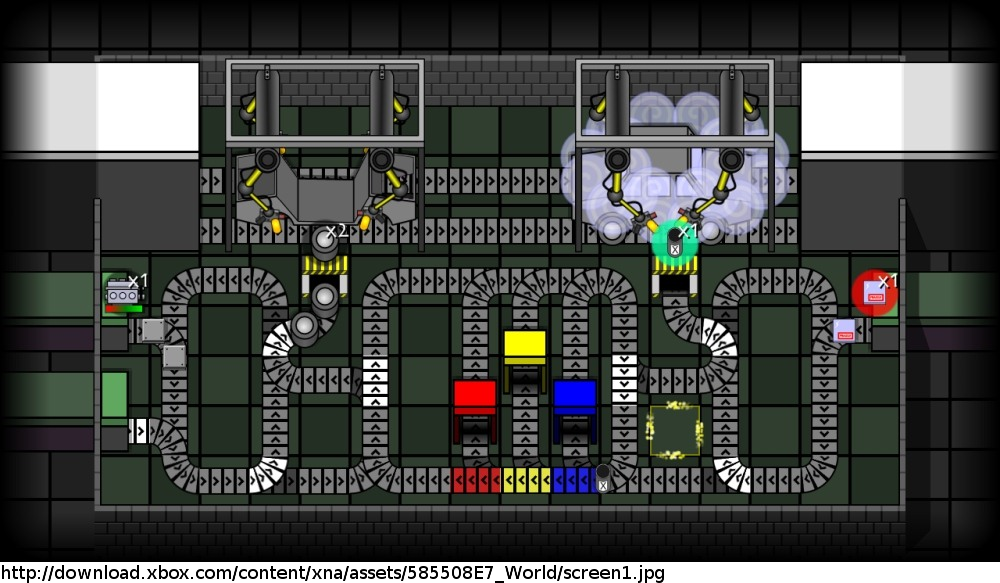
\includegraphics[width=0.49\textwidth]{similar_games/ProductionPanic}
    \end{multicols}

    \begin{multicols}{2}
        \subsection{Candy Factory - LeeGT}
            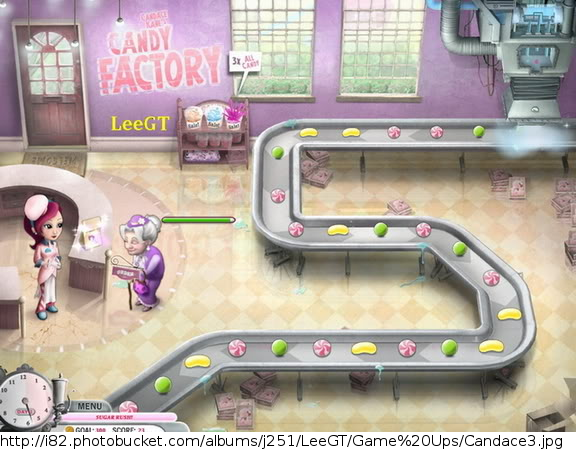
\includegraphics[width=0.49\textwidth]{similar_games/CandyFactoryLeeGT}

        \subsection{Teddy Factory}
            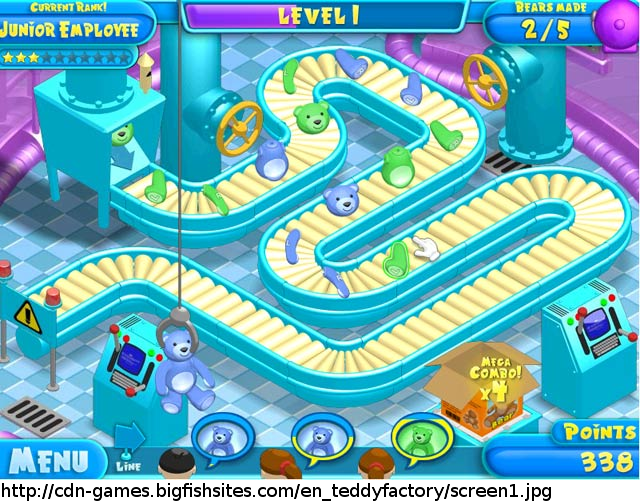
\includegraphics[width=0.49\textwidth]{similar_games/TeddyFactory}
    \end{multicols}

    \begin{multicols}{2}
        \subsection{Robot Factory}
            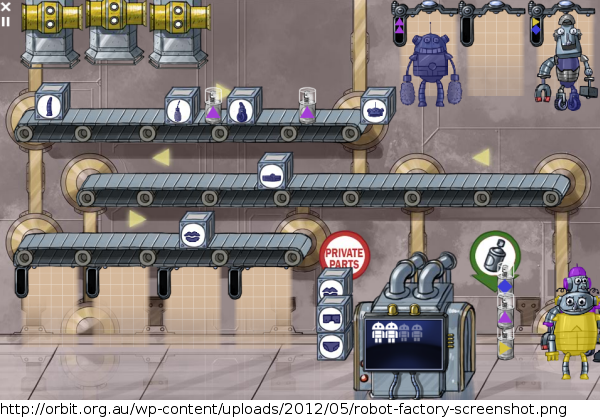
\includegraphics[width=0.49\textwidth]{similar_games/RobotFactory}

        \subsection{Space Chem}
            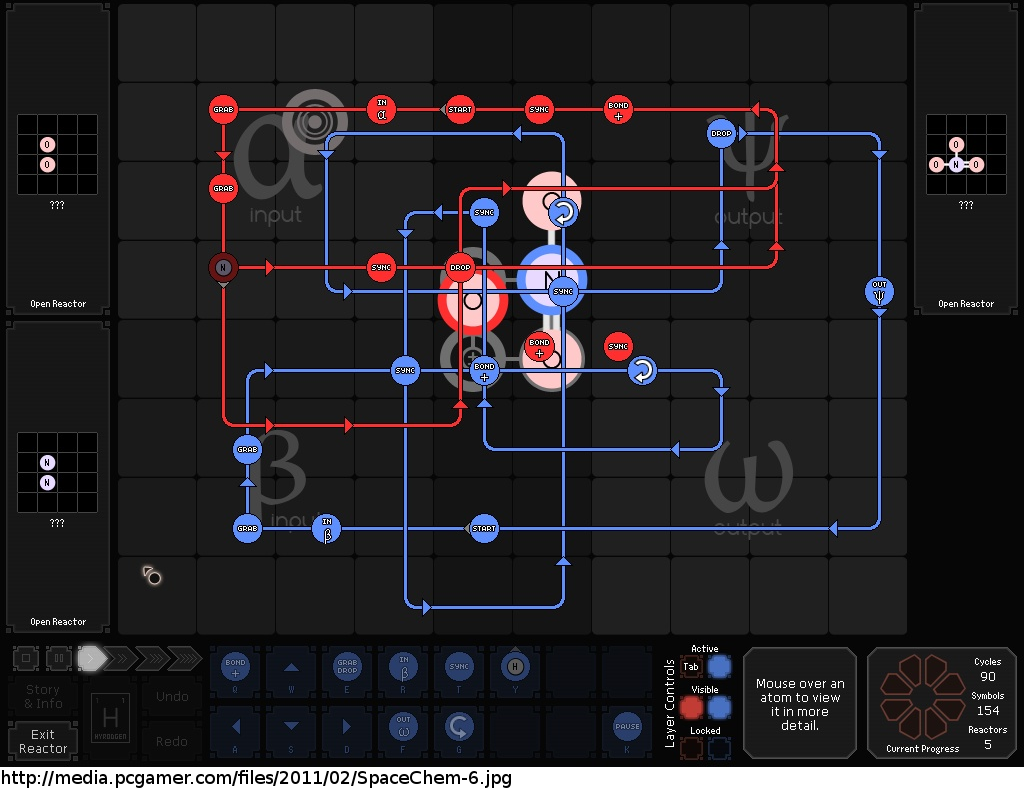
\includegraphics[width=0.49\textwidth]{similar_games/SpaceChem}
    \end{multicols}

\section{Game name alternatives}
    \begin{itemize}
        \item Smart Factory
        \item Smart Cream
        \item Smart Ice Cream Factory
        \item Smart Split
        \item Ice Cream Factory
    \end{itemize}

\end{document}
